% =====================================================================
%  Proyecto 13 · Clasificación de actividades humanas (UCI HAR) · Springer LNCS
%  Autor: Joan David Martínez Hernández
%  Plantilla: LLNCS 2.21 (estructura heredada de Springer_plantilla.tex)
%  Trazabilidad: cada cifra lleva un comentario %EXP-xxx que remite a
%  registro_experimentos.csv o al archivo de resultados de origen.
% =====================================================================
\documentclass[runningheads]{llncs}
%
\usepackage[T1]{fontenc}
\usepackage[utf8]{inputenc}
\usepackage[spanish,es-tabla,es-nodecimaldot]{babel}
\usepackage{graphicx}
\usepackage{booktabs}
\usepackage{array}
\usepackage{amsmath}
\usepackage{amssymb}
\usepackage{multirow}
\usepackage{orcidlink}
\usepackage{float}
\usepackage{tikz}
\usetikzlibrary{positioning,arrows.meta,calc,fit}
\usepackage{hyperref}
%
\usepackage{color}
\renewcommand\UrlFont{\color{blue}\rmfamily}
\renewcommand{\keywordname}{\textbf{Palabras clave:}}
\renewcommand{\orcidID}[1]{\textsuperscript{\scriptsize\orcidlink{#1}}}
\AtBeginDocument{\renewcommand{\tablename}{Tabla}%
\renewcommand{\figurename}{Fig.}\renewcommand{\refname}{Referencias}}
\addto\captionsspanish{\renewcommand{\refname}{Referencias}}
\setlength{\textfloatsep}{8pt}
\setlength{\intextsep}{8pt}
\providecommand{\doi}[1]{\href{https://doi.org/#1}{https://doi.org/#1}}
\newcommand{\pmv}[2]{#1\,{\scriptsize$\pm$\,#2}}   % media ± desv. est.
%
\raggedbottom   % evita estirar el espacio vertical cuando un float se fija con [H]
\begin{document}
%
\title{Reconocimiento de actividades humanas con redes LSTM sobre señales inerciales crudas y evaluación independiente del sujeto}
\titlerunning{Reconocimiento de actividades humanas con redes LSTM}
%
\author{Joan D. Martínez-Hernández\orcidID{0009-0002-2610-4441}}
\authorrunning{J.D. Martínez-Hernández}
\institute{Facultad de Ciencias Básicas e Ingeniería,
Universidad de los Llanos, Villavicencio, Colombia\\
\email{joan.martinez@unillanos.edu.co}}
%
\maketitle
%
% ---------------------------------------------------------------- RESUMEN
\begin{abstract}
El reconocimiento automático de actividades humanas a partir de los sensores
inerciales de un teléfono inteligente tiene aplicaciones en salud, deporte y
dispositivos vestibles. Este trabajo compara dos arquitecturas recurrentes, una
LSTM apilada y una variante Conv1D+LSTM, que clasifican seis actividades
directamente a partir de ventanas de 2,56\,s con nueve señales inerciales crudas
del conjunto UCI HAR (30 sujetos). Siguiendo CRISP-DM y para estimar el
desempeño sobre personas no vistas, la partición, la normalización y la
validación cruzada de dos particiones (repetida con tres semillas) se hicieron
por sujeto, y los experimentos se registraron en Weights \& Biases. Ambas arquitecturas
alcanzaron una exactitud media de 0,892 en validación cruzada (desviación
estándar de 0,037 y 0,064) y la diferencia no fue significativa según la
prueba $t$ corregida de Nadeau y Bengio, por lo que se eligió la LSTM por
parsimonia. El modelo final obtuvo una exactitud de 0,910\,$\pm$\,0,016 en
validación con cuatro sujetos reservados y de 0,914 en la partición oficial de
prueba (nueve sujetos). El error dominante fue la confusión entre estar de pie y
sentado, concentrada en pocos sujetos y asociada a la inclinación del teléfono;
además, se identificó una orientación de reposo ausente en el entrenamiento.
Se desarrolló una interfaz en Streamlit que muestra la actividad predicha y la
distribución de probabilidad por clase.
%
\keywords{Reconocimiento de actividades humanas \and Señales inerciales \and
LSTM \and Validación por sujeto \and Aprendizaje profundo.}
\end{abstract}
%
% ---------------------------------------------------------------- 1. INTRODUCCIÓN
\section{Introducción}

Los teléfonos inteligentes integran acelerómetros y giroscopios que permiten
reconocer, sin instrumentación adicional, actividades cotidianas como caminar,
subir escaleras o permanecer sentado. Este reconocimiento (HAR, por sus siglas
en inglés) es la base de aplicaciones de monitoreo de la salud, del
entrenamiento deportivo y de dispositivos vestibles. El conjunto UCI HAR se
publicó con un vector de 561 características diseñadas a mano y una línea base
basada en máquinas de vectores de soporte~\cite{anguita2013}. El aprendizaje
profundo permite, en cambio, aprender la representación directamente desde la
señal: las redes LSTM~\cite{hochreiter1997} modelan dependencias temporales, y
la arquitectura DeepConvLSTM combina capas convolucionales y recurrentes para
extraer características y modelar su evolución~\cite{ordonez2016}. Sin embargo,
el beneficio de las capas recurrentes depende del tipo de actividad y del
conjunto de datos~\cite{hammerla2016}, y en DeepConvLSTM una sola capa LSTM
supera a dos en cuatro de cinco conjuntos de referencia~\cite{bock2022}.

El problema abordado es doble. Primero, las ventanas de UCI HAR se solapan en un
50\,\% y la variabilidad entre personas es alta, de modo que una partición
aleatoria por ventana mezcla datos de un mismo sujeto en entrenamiento y
evaluación y sobrestima el desempeño. Segundo, comparar arquitecturas con pocas
particiones exige pruebas que tengan en cuenta la dependencia entre
evaluaciones~\cite{nadeau2003}. Este trabajo responde a la pregunta: ¿qué tan
bien clasifican dos arquitecturas recurrentes ligeras las actividades de
\emph{personas no vistas} a partir de señales crudas, y cuáles son sus errores
característicos? Se aporta un flujo reproducible con partición por sujeto y
trazabilidad en Weights \& Biases (W\&B), una comparación de arquitecturas con
validación cruzada repetida y prueba corregida, un análisis de errores por sujeto
y una interfaz de predicción.

% ---------------------------------------------------------------- 2. METODOLOGÍA
\section{Metodología}

El trabajo siguió las fases de CRISP-DM (entendimiento del problema y de los
datos, preparación, modelado, evaluación y despliegue). La
Fig.~\ref{fig:esquema} resume el sistema: cada ventana (128 pasos $\times$ 9
canales) se estandariza por canal y se clasifica con una red recurrente cuya
salida \emph{softmax} da la probabilidad de cada actividad.

\begin{figure}[H]
\centering
\begin{tikzpicture}[
  node distance=6mm and 4.2mm,
  box/.style={draw=black!45, rounded corners=2pt, fill=#1, align=center,
              font=\scriptsize, text width=25mm, minimum height=12mm, inner sep=2pt},
  box/.default=black!4,
  arr/.style={-{Stealth[length=1.6mm]}, draw=black!60, line width=.5pt}]
\node[box=teal!8] (d) {\textbf{UCI HAR}\\ 9 canales $\times$ 128\\ (2,56\,s a 50\,Hz)};
\node[box, right=of d] (p) {\textbf{Partición por sujeto}\\ DEV 17 · \mbox{HOLD-OUT} 4\\ TEST 9};
\node[box, right=of p] (n) {\textbf{Normalización $z$}\\ por canal, ajustada\\ con entrenamiento};
\node[box=teal!8, right=of n] (m) {\textbf{Modelos}\\ LSTM (64$\to$32)\\ Conv1D+LSTM};
\node[box, below=of m] (cv) {\textbf{Validación cruzada}\\ 2 particiones\\ $\times$ 3 semillas};
\node[box, left=of cv] (f) {\textbf{Modelo final}\\ LSTM en DEV\\ (7 épocas)};
\node[box, left=of f] (e) {\textbf{Evaluación}\\ HOLD-OUT (3 semillas)\\ TEST (única vez)};
\node[box=teal!8, left=of e] (ui) {\textbf{Interfaz}\\ Streamlit + D3\\ probabilidad por clase};
\draw[arr] (d)--(p); \draw[arr] (p)--(n); \draw[arr] (n)--(m); \draw[arr] (m)--(cv);
\draw[arr] (cv)--node[below,font=\tiny,yshift=-4.5mm]{}(f); \draw[arr] (f)--(e); \draw[arr] (e)--(ui);
\node[below=4mm of $(ui.south)!.5!(cv.south)$, anchor=north, draw=black!35, fill=black!3, rounded corners=2pt,
      font=\scriptsize, text width=11.6cm, align=center, inner sep=3pt] (wb)
  {\textbf{Weights \& Biases}: un experimento por (arquitectura, semilla, partición);
   métricas por época, matrices de confusión, modelos y estadísticos de normalización
   como artefactos; registro de experimentos EXP-001 a EXP-028};
\end{tikzpicture}
\caption{Esquema del sistema desarrollado: de las señales inerciales crudas a la
interfaz de predicción, con trazabilidad de todos los experimentos.}
\label{fig:esquema}
\end{figure}


\textbf{Arquitecturas.} (A) \emph{LSTM}: dos capas LSTM de 64 y 32 unidades,
cada una seguida de \emph{dropout} de 0,2, y una capa densa \emph{softmax}
(31\,558 parámetros). (B) \emph{Conv1D+LSTM}: dos convoluciones 1D de 64 filtros
(núcleo 5, ReLU), \emph{max-pooling} de factor 2, \emph{dropout} de 0,2, una capa
LSTM de 64 unidades y la capa \emph{softmax} (56\,902 parámetros). La variante B
sigue la idea de DeepConvLSTM~\cite{ordonez2016} con una sola capa
recurrente~\cite{bock2022}. Los tamaños se fijaron a priori, sin búsqueda de
hiperparámetros, por la restricción de cómputo (CPU Intel Core i5-1334U).

\textbf{Entrenamiento.} Se usó Adam con tasa de aprendizaje de $10^{-3}$, lotes
de 64, entropía cruzada categórica, un máximo de 50 épocas y parada temprana
sobre la pérdida de validación (paciencia de 8 épocas, restaurando los mejores
pesos). Se fijaron las semillas de Python, NumPy y TensorFlow, se activaron las
operaciones deterministas y se desactivaron las optimizaciones oneDNN
(TensorFlow 2.21, Keras 3.15).

% ---------------------------------------------------------------- 3. CONJUNTO DE DATOS
\section{Conjunto de datos}

UCI HAR~\cite{anguita2013,reyesortiz2012} contiene registros de 30 voluntarios de
19 a 48 años que realizaron seis actividades (caminar, subir escaleras, bajar
escaleras, sentado, de pie y acostado) con un Samsung Galaxy~S~II en la cintura.
Las señales del acelerómetro y del giroscopio se muestrearon a 50\,Hz, se
filtraron y se segmentaron en ventanas de 2,56\,s (128 muestras) con 50\,\% de
solapamiento; la aceleración total se separó en componentes corporal y de
gravedad mediante un filtro Butterworth paso bajo de 0,3\,Hz. La partición
oficial asigna 21 sujetos (7\,352 ventanas) a entrenamiento y 9 sujetos (2\,947
ventanas) a prueba. Se usaron las nueve señales crudas
(\texttt{body\_acc}, \texttt{body\_gyro} y \texttt{total\_acc} en los ejes $x$,
$y$, $z$), no las 561 características.

\begin{figure}[H]
\centering
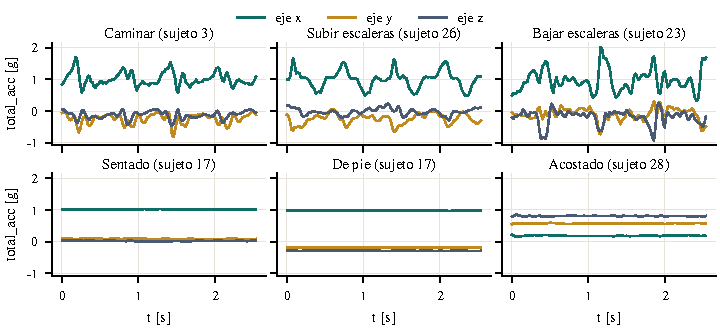
\includegraphics[width=\textwidth]{figuras/fig_datos.pdf}
\caption{Aceleración total (ejes $x$, $y$, $z$) en una ventana de cada actividad
del conjunto de entrenamiento.}
\label{fig:datos}
\end{figure}

El análisis exploratorio verificó el preprocesamiento declarado: no hay valores
faltantes ni ventanas duplicadas; el 95\,\% de las ventanas consecutivas de un
mismo sujeto y actividad comparte exactamente 64 muestras; y el módulo de la
gravedad estimada (\texttt{total\_acc}$-$\texttt{body\_acc}) es de
1,023\,$\pm$\,0,013\,g. Las señales, en cambio, no están normalizadas: la
desviación estándar varía hasta 3,9 veces entre canales. Las clases están
ligeramente desbalanceadas (razón máxima/mínima de 1,43) y cada sujeto aporta
entre 281 y 409 ventanas. Dentro de las actividades dinámicas, el sujeto explica
entre el 66\,\% y el 82\,\% de la varianza de la intensidad del movimiento y de la
orientación ($\eta^2$), lo que motiva la evaluación por sujeto. La
Fig.~\ref{fig:datos} muestra un ejemplo de cada actividad: las dinámicas
presentan oscilaciones periódicas, mientras que las estáticas se distinguen sobre
todo por la proyección de la gravedad sobre los ejes del teléfono.


% ---------------------------------------------------------------- 4. DISEÑO EXPERIMENTAL
\section{Diseño experimental}

\textbf{Partición.} La Fig.~\ref{fig:particion} resume el protocolo. Se conservó la
partición oficial de prueba (TEST) y del entrenamiento oficial se reservaron 4
sujetos como validación final (HOLD-OUT) con \texttt{StratifiedGroupKFold}
(5 grupos, semilla 42); los 17 restantes (DEV) se usaron en una validación
cruzada estratificada de dos particiones, repetida con tres semillas que cambian
el reparto de sujetos y la inicialización (seis evaluaciones por arquitectura).
Aserciones automáticas verificaron que ningún sujeto aparece en dos conjuntos, y
la proporción de cada clase difiere a lo sumo 1,54 puntos porcentuales entre
particiones. La normalización $z$ se ajustó solo con el entrenamiento de cada
partición.

\begin{figure}[H]
\centering
\begin{tikzpicture}[font=\scriptsize]
\definecolor{tealA}{HTML}{0E6E66}\definecolor{tealB}{HTML}{A9D3CE}\definecolor{ocre}{HTML}{C08A1E}
\definecolor{gris}{HTML}{8C9096}\definecolor{trn}{HTML}{DCE7EE}\definecolor{dev}{HTML}{7D8CA3}
\draw[black!50] (2.070,0.62) -- (2.070,0.68) -- (7.215,0.68) -- (7.215,0.62);
\node[anchor=south, inner sep=1pt] at (4.643,0.68) {\textbf{DEV: 17 sujetos}};
\draw[black!50] (7.415,0.62) -- (7.415,0.68) -- (8.595,0.68) -- (8.595,0.62);
\node[anchor=south, inner sep=1pt] at (8.005,0.68) {\textbf{{\tiny HOLD-OUT}}};
\draw[black!50] (8.795,0.62) -- (8.795,0.68) -- (11.500,0.68) -- (11.500,0.62);
\node[anchor=south, inner sep=1pt] at (10.148,0.68) {\textbf{TEST: 9 sujetos}};
\node[font=\tiny, text=black!60] at (2.202,0.42) {1};
\node[font=\tiny, text=black!60] at (2.507,0.42) {3};
\node[font=\tiny, text=black!60] at (2.812,0.42) {6};
\node[font=\tiny, text=black!60] at (3.117,0.42) {8};
\node[font=\tiny, text=black!60] at (3.422,0.42) {11};
\node[font=\tiny, text=black!60] at (3.727,0.42) {14};
\node[font=\tiny, text=black!60] at (4.032,0.42) {15};
\node[font=\tiny, text=black!60] at (4.337,0.42) {16};
\node[font=\tiny, text=black!60] at (4.643,0.42) {17};
\node[font=\tiny, text=black!60] at (4.947,0.42) {19};
\node[font=\tiny, text=black!60] at (5.252,0.42) {21};
\node[font=\tiny, text=black!60] at (5.557,0.42) {23};
\node[font=\tiny, text=black!60] at (5.862,0.42) {26};
\node[font=\tiny, text=black!60] at (6.167,0.42) {27};
\node[font=\tiny, text=black!60] at (6.472,0.42) {28};
\node[font=\tiny, text=black!60] at (6.777,0.42) {29};
\node[font=\tiny, text=black!60] at (7.082,0.42) {30};
\node[font=\tiny, text=black!60] at (7.547,0.42) {5};
\node[font=\tiny, text=black!60] at (7.853,0.42) {7};
\node[font=\tiny, text=black!60] at (8.157,0.42) {22};
\node[font=\tiny, text=black!60] at (8.462,0.42) {25};
\node[font=\tiny, text=black!60] at (8.928,0.42) {2};
\node[font=\tiny, text=black!60] at (9.232,0.42) {4};
\node[font=\tiny, text=black!60] at (9.537,0.42) {9};
\node[font=\tiny, text=black!60] at (9.843,0.42) {10};
\node[font=\tiny, text=black!60] at (10.148,0.42) {12};
\node[font=\tiny, text=black!60] at (10.453,0.42) {13};
\node[font=\tiny, text=black!60] at (10.758,0.42) {18};
\node[font=\tiny, text=black!60] at (11.062,0.42) {20};
\node[font=\tiny, text=black!60] at (11.367,0.42) {24};
\node[anchor=east, align=right] at (1.970,0.000) {Partición oficial};
\fill[trn] (2.062,-0.180) rectangle (2.343,0.180);
\fill[trn] (2.367,-0.180) rectangle (2.648,0.180);
\fill[trn] (2.672,-0.180) rectangle (2.953,0.180);
\fill[trn] (2.977,-0.180) rectangle (3.258,0.180);
\fill[trn] (3.282,-0.180) rectangle (3.563,0.180);
\fill[trn] (3.587,-0.180) rectangle (3.868,0.180);
\fill[trn] (3.892,-0.180) rectangle (4.173,0.180);
\fill[trn] (4.197,-0.180) rectangle (4.478,0.180);
\fill[trn] (4.502,-0.180) rectangle (4.783,0.180);
\fill[trn] (4.807,-0.180) rectangle (5.088,0.180);
\fill[trn] (5.112,-0.180) rectangle (5.393,0.180);
\fill[trn] (5.417,-0.180) rectangle (5.698,0.180);
\fill[trn] (5.722,-0.180) rectangle (6.003,0.180);
\fill[trn] (6.027,-0.180) rectangle (6.308,0.180);
\fill[trn] (6.332,-0.180) rectangle (6.613,0.180);
\fill[trn] (6.637,-0.180) rectangle (6.918,0.180);
\fill[trn] (6.942,-0.180) rectangle (7.223,0.180);
\fill[trn] (7.407,-0.180) rectangle (7.688,0.180);
\fill[trn] (7.712,-0.180) rectangle (7.993,0.180);
\fill[trn] (8.017,-0.180) rectangle (8.298,0.180);
\fill[trn] (8.322,-0.180) rectangle (8.603,0.180);
\fill[gris] (8.787,-0.180) rectangle (9.068,0.180);
\fill[gris] (9.092,-0.180) rectangle (9.373,0.180);
\fill[gris] (9.397,-0.180) rectangle (9.678,0.180);
\fill[gris] (9.702,-0.180) rectangle (9.983,0.180);
\fill[gris] (10.007,-0.180) rectangle (10.288,0.180);
\fill[gris] (10.312,-0.180) rectangle (10.593,0.180);
\fill[gris] (10.617,-0.180) rectangle (10.898,0.180);
\fill[gris] (10.922,-0.180) rectangle (11.203,0.180);
\fill[gris] (11.227,-0.180) rectangle (11.508,0.180);
\node[anchor=east, align=right] at (1.970,-0.430) {Reserva};
\fill[dev] (2.062,-0.610) rectangle (2.343,-0.250);
\fill[dev] (2.367,-0.610) rectangle (2.648,-0.250);
\fill[dev] (2.672,-0.610) rectangle (2.953,-0.250);
\fill[dev] (2.977,-0.610) rectangle (3.258,-0.250);
\fill[dev] (3.282,-0.610) rectangle (3.563,-0.250);
\fill[dev] (3.587,-0.610) rectangle (3.868,-0.250);
\fill[dev] (3.892,-0.610) rectangle (4.173,-0.250);
\fill[dev] (4.197,-0.610) rectangle (4.478,-0.250);
\fill[dev] (4.502,-0.610) rectangle (4.783,-0.250);
\fill[dev] (4.807,-0.610) rectangle (5.088,-0.250);
\fill[dev] (5.112,-0.610) rectangle (5.393,-0.250);
\fill[dev] (5.417,-0.610) rectangle (5.698,-0.250);
\fill[dev] (5.722,-0.610) rectangle (6.003,-0.250);
\fill[dev] (6.027,-0.610) rectangle (6.308,-0.250);
\fill[dev] (6.332,-0.610) rectangle (6.613,-0.250);
\fill[dev] (6.637,-0.610) rectangle (6.918,-0.250);
\fill[dev] (6.942,-0.610) rectangle (7.223,-0.250);
\fill[ocre] (7.407,-0.610) rectangle (7.688,-0.250);
\fill[ocre] (7.712,-0.610) rectangle (7.993,-0.250);
\fill[ocre] (8.017,-0.610) rectangle (8.298,-0.250);
\fill[ocre] (8.322,-0.610) rectangle (8.603,-0.250);
\fill[gris] (8.787,-0.610) rectangle (9.068,-0.250);
\fill[gris] (9.092,-0.610) rectangle (9.373,-0.250);
\fill[gris] (9.397,-0.610) rectangle (9.678,-0.250);
\fill[gris] (9.702,-0.610) rectangle (9.983,-0.250);
\fill[gris] (10.007,-0.610) rectangle (10.288,-0.250);
\fill[gris] (10.312,-0.610) rectangle (10.593,-0.250);
\fill[gris] (10.617,-0.610) rectangle (10.898,-0.250);
\fill[gris] (10.922,-0.610) rectangle (11.203,-0.250);
\fill[gris] (11.227,-0.610) rectangle (11.508,-0.250);
\node[anchor=east, align=right] at (1.970,-0.860) {VC, semilla 42};
\fill[tealB] (2.062,-1.040) rectangle (2.343,-0.680);
\fill[tealB] (2.367,-1.040) rectangle (2.648,-0.680);
\fill[tealB] (2.672,-1.040) rectangle (2.953,-0.680);
\fill[tealA] (2.977,-1.040) rectangle (3.258,-0.680);
\fill[tealB] (3.282,-1.040) rectangle (3.563,-0.680);
\fill[tealA] (3.587,-1.040) rectangle (3.868,-0.680);
\fill[tealB] (3.892,-1.040) rectangle (4.173,-0.680);
\fill[tealB] (4.197,-1.040) rectangle (4.478,-0.680);
\fill[tealA] (4.502,-1.040) rectangle (4.783,-0.680);
\fill[tealB] (4.807,-1.040) rectangle (5.088,-0.680);
\fill[tealA] (5.112,-1.040) rectangle (5.393,-0.680);
\fill[tealA] (5.417,-1.040) rectangle (5.698,-0.680);
\fill[tealA] (5.722,-1.040) rectangle (6.003,-0.680);
\fill[tealA] (6.027,-1.040) rectangle (6.308,-0.680);
\fill[tealA] (6.332,-1.040) rectangle (6.613,-0.680);
\fill[tealA] (6.637,-1.040) rectangle (6.918,-0.680);
\fill[tealB] (6.942,-1.040) rectangle (7.223,-0.680);
\draw[black!20, line width=.3pt] (7.425,-0.860) -- (7.670,-0.860);
\draw[black!20, line width=.3pt] (7.730,-0.860) -- (7.975,-0.860);
\draw[black!20, line width=.3pt] (8.035,-0.860) -- (8.280,-0.860);
\draw[black!20, line width=.3pt] (8.340,-0.860) -- (8.585,-0.860);
\draw[black!20, line width=.3pt] (8.805,-0.860) -- (9.050,-0.860);
\draw[black!20, line width=.3pt] (9.110,-0.860) -- (9.355,-0.860);
\draw[black!20, line width=.3pt] (9.415,-0.860) -- (9.660,-0.860);
\draw[black!20, line width=.3pt] (9.720,-0.860) -- (9.965,-0.860);
\draw[black!20, line width=.3pt] (10.025,-0.860) -- (10.270,-0.860);
\draw[black!20, line width=.3pt] (10.330,-0.860) -- (10.575,-0.860);
\draw[black!20, line width=.3pt] (10.635,-0.860) -- (10.880,-0.860);
\draw[black!20, line width=.3pt] (10.940,-0.860) -- (11.185,-0.860);
\draw[black!20, line width=.3pt] (11.245,-0.860) -- (11.490,-0.860);
\node[anchor=east, align=right] at (1.970,-1.290) {VC, semilla 43};
\fill[tealB] (2.062,-1.470) rectangle (2.343,-1.110);
\fill[tealB] (2.367,-1.470) rectangle (2.648,-1.110);
\fill[tealB] (2.672,-1.470) rectangle (2.953,-1.110);
\fill[tealA] (2.977,-1.470) rectangle (3.258,-1.110);
\fill[tealA] (3.282,-1.470) rectangle (3.563,-1.110);
\fill[tealB] (3.587,-1.470) rectangle (3.868,-1.110);
\fill[tealA] (3.892,-1.470) rectangle (4.173,-1.110);
\fill[tealB] (4.197,-1.470) rectangle (4.478,-1.110);
\fill[tealA] (4.502,-1.470) rectangle (4.783,-1.110);
\fill[tealA] (4.807,-1.470) rectangle (5.088,-1.110);
\fill[tealA] (5.112,-1.470) rectangle (5.393,-1.110);
\fill[tealA] (5.417,-1.470) rectangle (5.698,-1.110);
\fill[tealA] (5.722,-1.470) rectangle (6.003,-1.110);
\fill[tealB] (6.027,-1.470) rectangle (6.308,-1.110);
\fill[tealB] (6.332,-1.470) rectangle (6.613,-1.110);
\fill[tealB] (6.637,-1.470) rectangle (6.918,-1.110);
\fill[tealA] (6.942,-1.470) rectangle (7.223,-1.110);
\draw[black!20, line width=.3pt] (7.425,-1.290) -- (7.670,-1.290);
\draw[black!20, line width=.3pt] (7.730,-1.290) -- (7.975,-1.290);
\draw[black!20, line width=.3pt] (8.035,-1.290) -- (8.280,-1.290);
\draw[black!20, line width=.3pt] (8.340,-1.290) -- (8.585,-1.290);
\draw[black!20, line width=.3pt] (8.805,-1.290) -- (9.050,-1.290);
\draw[black!20, line width=.3pt] (9.110,-1.290) -- (9.355,-1.290);
\draw[black!20, line width=.3pt] (9.415,-1.290) -- (9.660,-1.290);
\draw[black!20, line width=.3pt] (9.720,-1.290) -- (9.965,-1.290);
\draw[black!20, line width=.3pt] (10.025,-1.290) -- (10.270,-1.290);
\draw[black!20, line width=.3pt] (10.330,-1.290) -- (10.575,-1.290);
\draw[black!20, line width=.3pt] (10.635,-1.290) -- (10.880,-1.290);
\draw[black!20, line width=.3pt] (10.940,-1.290) -- (11.185,-1.290);
\draw[black!20, line width=.3pt] (11.245,-1.290) -- (11.490,-1.290);
\node[anchor=east, align=right] at (1.970,-1.720) {VC, semilla 44};
\fill[tealA] (2.062,-1.900) rectangle (2.343,-1.540);
\fill[tealB] (2.367,-1.900) rectangle (2.648,-1.540);
\fill[tealA] (2.672,-1.900) rectangle (2.953,-1.540);
\fill[tealA] (2.977,-1.900) rectangle (3.258,-1.540);
\fill[tealB] (3.282,-1.900) rectangle (3.563,-1.540);
\fill[tealA] (3.587,-1.900) rectangle (3.868,-1.540);
\fill[tealB] (3.892,-1.900) rectangle (4.173,-1.540);
\fill[tealA] (4.197,-1.900) rectangle (4.478,-1.540);
\fill[tealB] (4.502,-1.900) rectangle (4.783,-1.540);
\fill[tealA] (4.807,-1.900) rectangle (5.088,-1.540);
\fill[tealA] (5.112,-1.900) rectangle (5.393,-1.540);
\fill[tealB] (5.417,-1.900) rectangle (5.698,-1.540);
\fill[tealA] (5.722,-1.900) rectangle (6.003,-1.540);
\fill[tealB] (6.027,-1.900) rectangle (6.308,-1.540);
\fill[tealB] (6.332,-1.900) rectangle (6.613,-1.540);
\fill[tealB] (6.637,-1.900) rectangle (6.918,-1.540);
\fill[tealA] (6.942,-1.900) rectangle (7.223,-1.540);
\draw[black!20, line width=.3pt] (7.425,-1.720) -- (7.670,-1.720);
\draw[black!20, line width=.3pt] (7.730,-1.720) -- (7.975,-1.720);
\draw[black!20, line width=.3pt] (8.035,-1.720) -- (8.280,-1.720);
\draw[black!20, line width=.3pt] (8.340,-1.720) -- (8.585,-1.720);
\draw[black!20, line width=.3pt] (8.805,-1.720) -- (9.050,-1.720);
\draw[black!20, line width=.3pt] (9.110,-1.720) -- (9.355,-1.720);
\draw[black!20, line width=.3pt] (9.415,-1.720) -- (9.660,-1.720);
\draw[black!20, line width=.3pt] (9.720,-1.720) -- (9.965,-1.720);
\draw[black!20, line width=.3pt] (10.025,-1.720) -- (10.270,-1.720);
\draw[black!20, line width=.3pt] (10.330,-1.720) -- (10.575,-1.720);
\draw[black!20, line width=.3pt] (10.635,-1.720) -- (10.880,-1.720);
\draw[black!20, line width=.3pt] (10.940,-1.720) -- (11.185,-1.720);
\draw[black!20, line width=.3pt] (11.245,-1.720) -- (11.490,-1.720);
\node[anchor=west, inner sep=0pt] (lg00) at (2.000,-2.250) {\textcolor{trn}{\rule{2.4mm}{2.4mm}}\,entrenamiento oficial};
\node[anchor=west, inner sep=0pt] (lg01) [right=3.2mm of lg00] {\textcolor{dev}{\rule{2.4mm}{2.4mm}}\,desarrollo (DEV)};
\node[anchor=west, inner sep=0pt] (lg02) [right=3.2mm of lg01] {\textcolor{ocre}{\rule{2.4mm}{2.4mm}}\,validación final (HOLD-OUT)};
\node[anchor=west, inner sep=0pt] (lg10) at (2.000,-2.610) {\textcolor{gris}{\rule{2.4mm}{2.4mm}}\,prueba oficial (TEST)};
\node[anchor=west, inner sep=0pt] (lg11) [right=3.2mm of lg10] {\textcolor{tealA}{\rule{2.4mm}{2.4mm}}\,partición A};
\node[anchor=west, inner sep=0pt] (lg12) [right=3.2mm of lg11] {\textcolor{tealB}{\rule{2.4mm}{2.4mm}}\,partición B};
\node[anchor=west, inner sep=0pt] (lg13) [right=3.2mm of lg12] {\textcolor{black!35}{\rule[.9mm]{2.4mm}{.4pt}}\,no participa};
\node[draw=black!45, rounded corners=2pt, align=center, text width=2.50cm, minimum height=1.45cm, inner sep=2pt, anchor=west, execute at begin node={\hyphenpenalty=10000\relax}, fill=tealB!40] (f0) at (0.000,-3.730) {\textbf{Cada semilla y partición:} $z$ y red ajustadas con A; exactitud en B, y al revés};
\node[draw=black!45, rounded corners=2pt, align=center, text width=2.50cm, minimum height=1.45cm, inner sep=2pt, anchor=west, execute at begin node={\hyphenpenalty=10000\relax}, fill=black!4] (f1) at (2.967,-3.730) {\textbf{6 exactitudes} por arquitectura: media $\pm$ DE; $t$ de \mbox{Nadeau--Bengio} $\to$ LSTM};
\node[draw=black!45, rounded corners=2pt, align=center, text width=2.50cm, minimum height=1.45cm, inner sep=2pt, anchor=west, execute at begin node={\hyphenpenalty=10000\relax}, fill=dev!18] (f2) at (5.933,-3.730) {\textbf{Modelo final:} LSTM en todo DEV (7~épocas; $z$ de DEV)};
\node[draw=black!45, rounded corners=2pt, align=center, text width=2.50cm, minimum height=1.45cm, inner sep=2pt, anchor=west, execute at begin node={\hyphenpenalty=10000\relax}, fill=ocre!18] (f3) at (8.900,-3.730) {\textbf{Evaluación:} HOLD-OUT, 3 semillas (c); TEST, una sola vez (d)};
\draw[-{Stealth[length=1.8mm]}, black!60] (f0.east) -- (f1.west);
\draw[-{Stealth[length=1.8mm]}, black!60] (f1.east) -- (f2.west);
\draw[-{Stealth[length=1.8mm]}, black!60] (f2.east) -- (f3.west);
\end{tikzpicture}

\caption{Partición por sujeto y validación cruzada (VC). Cada columna es un sujeto
de UCI HAR. Del entrenamiento oficial (21 sujetos) se reserva el HOLD-OUT (1\,340
ventanas) y quedan 17 sujetos en DEV (6\,012 ventanas); en cada semilla, los
sujetos de DEV se reparten en las particiones A y B, se entrena con una y se
valida con la otra. El TEST (2\,947 ventanas) solo se usa en la evaluación final.}
\label{fig:particion}
\end{figure}

El modelo final (LSTM) se entrenó con todo DEV durante 7 épocas fijas (mediana
de la mejor época en la validación cruzada), se evaluó en el HOLD-OUT
(``validación'' en el enunciado) con tres semillas, y el modelo de la semilla 42,
que usa la interfaz, se evaluó una única vez en el TEST.

\textbf{Medidas de desempeño.} Se reportan la exactitud, la precisión $P$, la
exhaustividad $R$ y $F_1=2PR/(P+R)$ por actividad y en promedio macro, junto con
la matriz de confusión, como media $\pm$ desviación estándar muestral cuando hay
varias corridas. Para comparar arquitecturas se usaron las seis diferencias
pareadas de exactitud $d_k$ con la prueba $t$ pareada, la de Wilcoxon y la $t$
corregida de Nadeau y Bengio~\cite{nadeau2003},
$t=\bar d\,/\sqrt{(1/n+n_2/n_1)\,s_d^2}$, con $n=6$ y $n_2/n_1\approx1$ para dos
particiones; esta corrección compensa la subestimación de la varianza que produce
el solapamiento entre conjuntos de entrenamiento. Como análisis de sensibilidad,
la validación cruzada se repitió con la parada temprana sobre la exactitud de
validación. Los 28 experimentos (EXP-001 a EXP-028) se registraron en W\&B.

% ---------------------------------------------------------------- 5. RESULTADOS
\section{Resultados}

\textbf{Selección de arquitectura.} La Tabla~\ref{tab:cv} resume la validación
cruzada. % EXP-001..EXP-012 (principal); EXP-013..EXP-024 (sensibilidad)
En el protocolo principal ambas arquitecturas obtuvieron la misma exactitud
media; la diferencia pareada fue de $-0{,}0005$ ($p=0{,}98$ con $t$ pareada,
$p=0{,}99$ con la corrección de Nadeau--Bengio y $p=0{,}625$ con Wilcoxon). La mayor dispersión de Conv1D+LSTM se debe a una corrida (semilla 43, partición
1) detenida por la pérdida en la primera época, con exactitud de 0,777; al parar
sobre la exactitud alcanzó 0,881. En el análisis de sensibilidad
Conv1D+LSTM fue mejor en cinco de seis pares (diferencia media de $+0{,}012$),
sin significancia ($p=0{,}20$; $p=0{,}60$ corregida; $p=0{,}31$ Wilcoxon), y
ese protocolo es optimista porque elige la época con la misma métrica que
reporta. Se eligió la LSTM por parsimonia: con un desempeño indistinguible,
Conv1D+LSTM añade un 80\,\% de parámetros e hiperparámetros de diseño. El
argumento no es el tiempo de cómputo, pues Conv1D+LSTM entrenó más rápido
(7--10\,s frente a 11--15\,s por época) gracias al \emph{pooling}.

\begin{table}[!b]
\centering
\caption{Validación cruzada por sujeto (2 particiones $\times$ 3 semillas, $n=6$):
media $\pm$ desviación estándar.}\label{tab:cv}
\footnotesize
\begin{tabular}{lrcccc}
\toprule
 & & \multicolumn{2}{c}{Principal (paro: pérdida)} & \multicolumn{2}{c}{Sensibilidad (paro: exactitud)}\\
\cmidrule(lr){3-4}\cmidrule(lr){5-6}
\textbf{Arquitectura} & \textbf{Parám.} & \textbf{Exactitud} & \textbf{F1 macro} & \textbf{Exactitud} & \textbf{F1 macro}\\
\midrule
LSTM        & 31\,558 & \pmv{0,892}{0,037} & \pmv{0,894}{0,037} & \pmv{0,908}{0,035} & \pmv{0,910}{0,034}\\
Conv1D+LSTM & 56\,902 & \pmv{0,892}{0,064} & \pmv{0,889}{0,075} & \pmv{0,920}{0,025} & \pmv{0,923}{0,025}\\
\midrule
\multicolumn{2}{l}{Diferencia (B$-$A); $p$ corregida} & $-$0,0005; 0,99 & & $+$0,012; 0,60 & \\
\bottomrule
\end{tabular}
\end{table}

\textbf{Modelo final en validación.} En el HOLD-OUT, la LSTM final alcanzó una
exactitud de 0,910\,$\pm$\,0,016 y un F1 macro de 0,911\,$\pm$\,0,015 con tres
semillas (Tabla~\ref{tab:clases}). % EXP-025..EXP-027
Las actividades dinámicas y \emph{acostado} superaron 0,96 de F1, mientras que
\emph{de pie} tuvo la menor exhaustividad (0,608): el 39\,\% de sus ventanas se
clasificó como \emph{sentado}, y la confusión inversa fue casi nula.

\begin{table}[t]
\centering
\caption{Métricas por actividad del modelo final. HOLD-OUT: 4 sujetos, media
$\pm$ desviación estándar de 3 semillas. TEST: 9 sujetos, modelo desplegado
(semilla 42), evaluación única.}\label{tab:clases}
\scriptsize
\setlength{\tabcolsep}{4pt}
\begin{tabular}{lccc@{\hspace{10pt}}ccc}
\toprule
 & \multicolumn{3}{c}{HOLD-OUT (validación)} & \multicolumn{3}{c}{TEST (prueba oficial)}\\
\cmidrule(lr){2-4}\cmidrule(lr){5-7}
\textbf{Actividad} & \textbf{Precisión} & \textbf{Exhaustividad} & \textbf{F1} & \textbf{Prec.} & \textbf{Exh.} & \textbf{F1}\\
\midrule
Caminar         & \pmv{0,975}{0,013} & \pmv{0,956}{0,026} & \pmv{0,965}{0,016} & 0,958 & 0,970 & 0,964\\
Subir escaleras & \pmv{0,973}{0,014} & \pmv{0,979}{0,012} & \pmv{0,976}{0,013} & 0,869 & 0,915 & 0,891\\
Bajar escaleras & \pmv{0,984}{0,014} & \pmv{0,966}{0,035} & \pmv{0,975}{0,020} & 0,936 & 0,971 & 0,953\\
Sentado         & \pmv{0,683}{0,042} & \pmv{0,988}{0,010} & \pmv{0,807}{0,028} & 0,819 & 0,864 & 0,840\\
De pie          & \pmv{0,987}{0,011} & \pmv{0,608}{0,042} & \pmv{0,752}{0,032} & 0,915 & 0,825 & 0,868\\
Acostado        & \pmv{0,988}{0,017} & \pmv{0,997}{0,005} & \pmv{0,993}{0,011} & 0,990 & 0,950 & 0,970\\
\midrule
Macro           & \pmv{0,932}{0,008} & \pmv{0,916}{0,016} & \pmv{0,911}{0,015} & 0,914 & 0,916 & 0,914\\
Exactitud       & \multicolumn{3}{c}{\pmv{0,910}{0,016}} & \multicolumn{3}{c}{0,914}\\
\bottomrule
\end{tabular}
\end{table}

\textbf{Prueba y análisis de errores.} En el TEST, el modelo desplegado obtuvo una
exactitud y un F1 macro de 0,914 (Tabla~\ref{tab:clases}), % EXP-028, W&B f8j4v23e
dentro del rango de la validación, sin indicios de sobreajuste a la selección
del modelo. La Tabla~\ref{tab:cm} muestra la matriz de confusión y la
Fig.~\ref{fig:ejemplos}, cinco aciertos y cinco errores elegidos con una regla
fijada de antemano (al azar con semilla 42; errores de los cinco pares más
frecuentes).

\begin{table}[t]
\centering
\caption{Matriz de confusión en el TEST (filas: actividad real; columnas:
predicha; 2\,947 ventanas).}\label{tab:cm}
\footnotesize
\begin{tabular}{lrrrrrr}
\toprule
\textbf{Real $\backslash$ Predicha} & \textbf{Caminar} & \textbf{Subir} & \textbf{Bajar} & \textbf{Sentado} & \textbf{De pie} & \textbf{Acostado}\\
\midrule
Caminar         & \textbf{481} & 7 & 8 & 0 & 0 & 0\\
Subir escaleras & 21 & \textbf{431} & 19 & 0 & 0 & 0\\
Bajar escaleras & 0 & 11 & \textbf{408} & 1 & 0 & 0\\
Sentado         & 0 & 20 & 1 & \textbf{424} & 41 & 5\\
De pie          & 0 & 0 & 0 & 93 & \textbf{439} & 0\\
Acostado        & 0 & 27 & 0 & 0 & 0 & \textbf{510}\\
\bottomrule
\end{tabular}
\end{table}

\begin{figure}[!t]
\centering
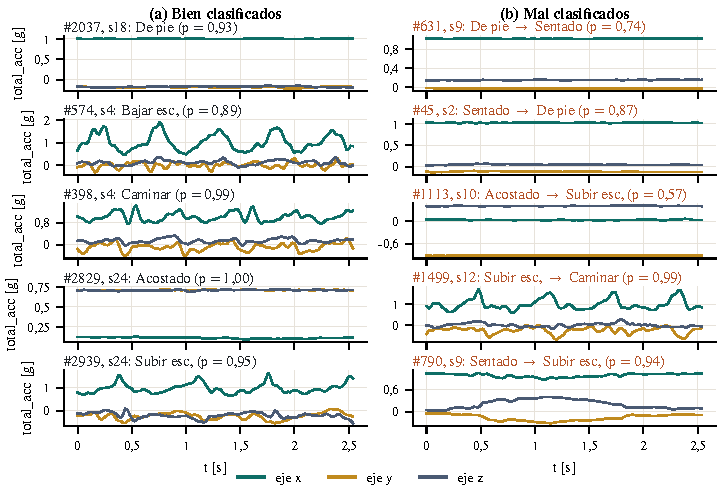
\includegraphics[width=\textwidth]{figuras/fig_ejemplos_test.pdf}
\caption{Ejemplos del TEST: aceleración total de cinco ventanas bien
clasificadas (a) y cinco mal clasificadas (b), con índice de ventana, sujeto,
actividad real $\rightarrow$ predicha y probabilidad asignada.}
\label{fig:ejemplos}
\end{figure}

La confusión entre \emph{sentado} y \emph{de pie} concentra 134 de los 254 errores
(53\,\%) y se limita a pocos sujetos: seis de los nueve sujetos de prueba tienen
una exhaustividad de 1,00 en \emph{de pie}, mientras que la del sujeto~9 es de
0,02. En ese sujeto, la componente $y$ media de la gravedad es prácticamente igual
de pie y sentado (0,008 y $-0{,}023$\,g), mientras que en DEV ambas posturas se
separan ($-0{,}173$ y $0{,}134$\,g; ejemplo \#631). Esto sugiere que el modelo
distingue ambas posturas sobre todo por la inclinación del teléfono, que varía con
la anatomía o la colocación del dispositivo; el patrón se repitió en el HOLD-OUT,
aunque con pocos sujetos no puede afirmarse una relación causal. Un
segundo modo de fallo es la orientación fuera de distribución: las 27 ventanas
de \emph{acostado} clasificadas como \emph{subir escaleras} pertenecen al
sujeto~10, cuya gravedad cae casi por completo en el eje $-y$
($\approx-0{,}93$\,g, ejemplo \#1113), un valor que no aparece en las ventanas de \emph{acostado} de DEV (mínimo
de $-0{,}48$\,g). Además, algunas ventanas estáticas
contienen movimiento (\#45, \#790), compatible con transiciones posturales no
etiquetadas, y \emph{subir escaleras} se confunde con \emph{caminar} (21
ventanas, \#1499), que comparten el pico espectral de 1,56\,Hz. La
exactitud por sujeto en el TEST va de 0,653 (sujeto~10) a 0,997 (sujeto~24). Las
probabilidades no están calibradas: la confianza media es de 0,945 en los aciertos
y de 0,789 en los errores, pero 100 de los 254 errores tienen una probabilidad
mayor de 0,9.

\textbf{Interfaz.} La aplicación en Streamlit (Fig.~\ref{fig:app}) carga una
ventana del TEST (elegida por actividad) o un CSV de 128$\times$9 en unidades
físicas, aplica la normalización del entrenamiento y muestra la actividad
predicha, la probabilidad por clase, la etiqueta real cuando existe, las señales
en gráficas D3 y una advertencia sobre la falta de calibración. Sus predicciones coinciden con la evaluación (\#631: \emph{sentado}, 0,744).

\begin{figure}[H]
\centering
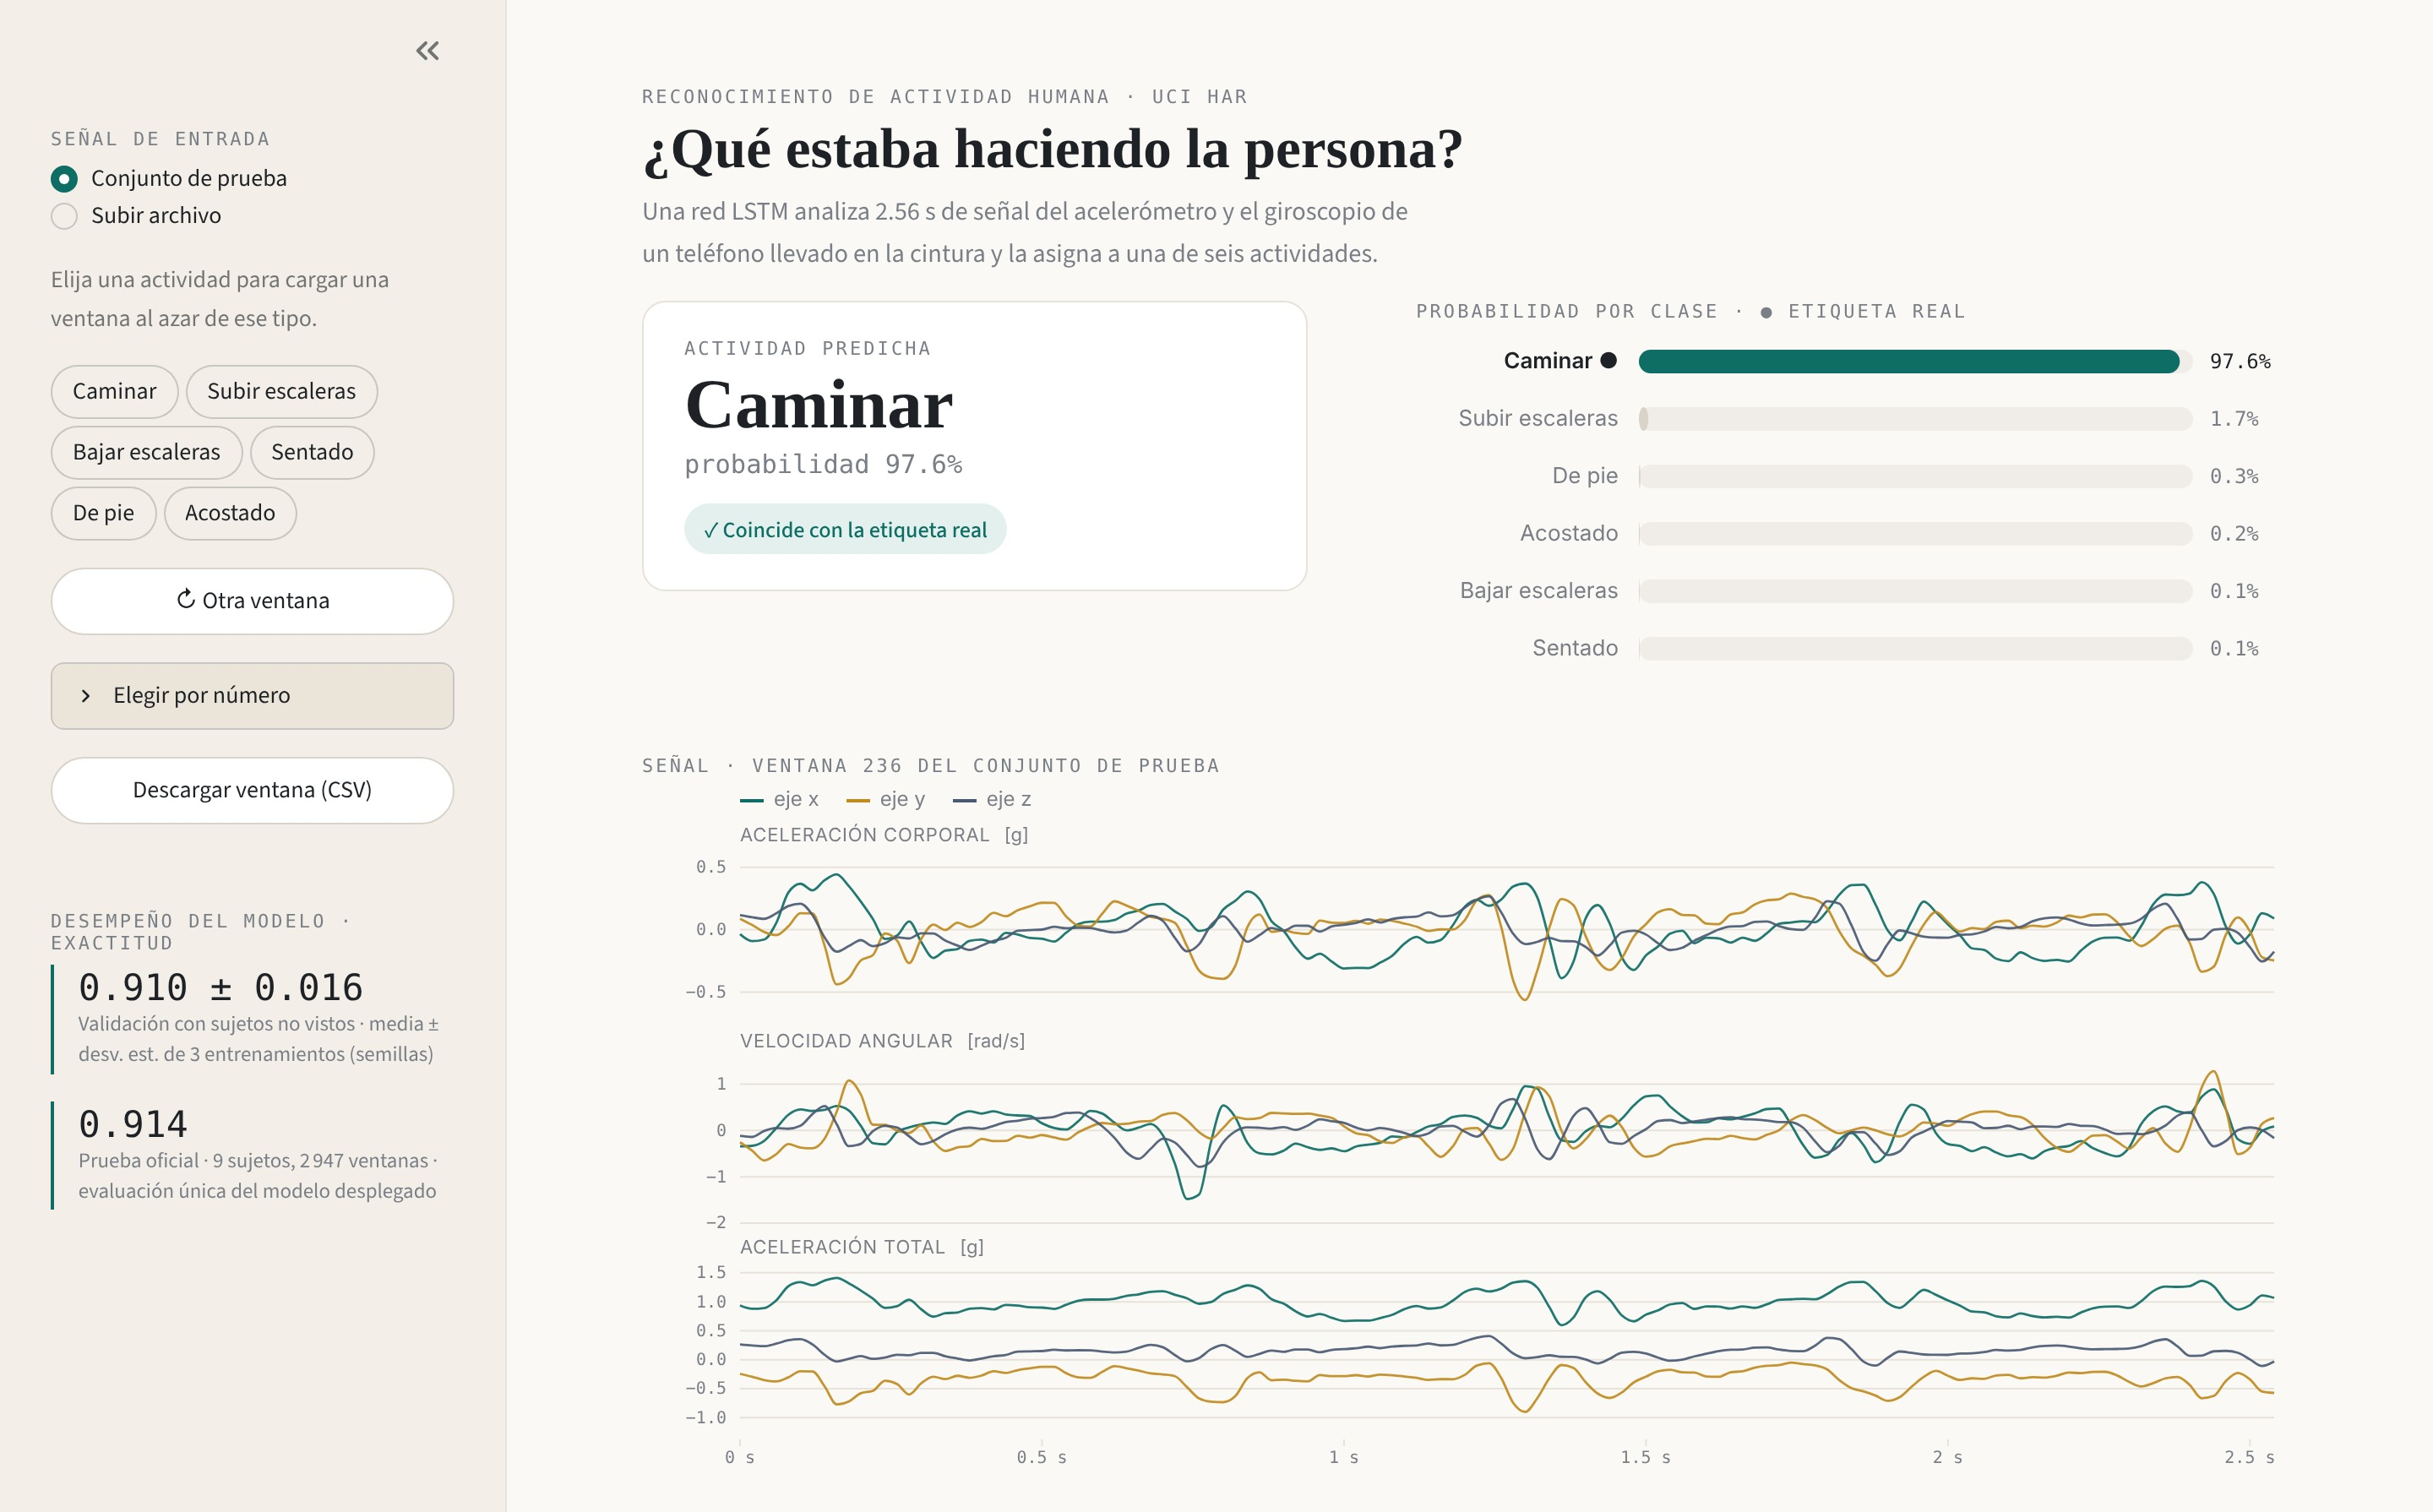
\includegraphics[width=.495\textwidth]{figuras/app_236.jpg}\hfill
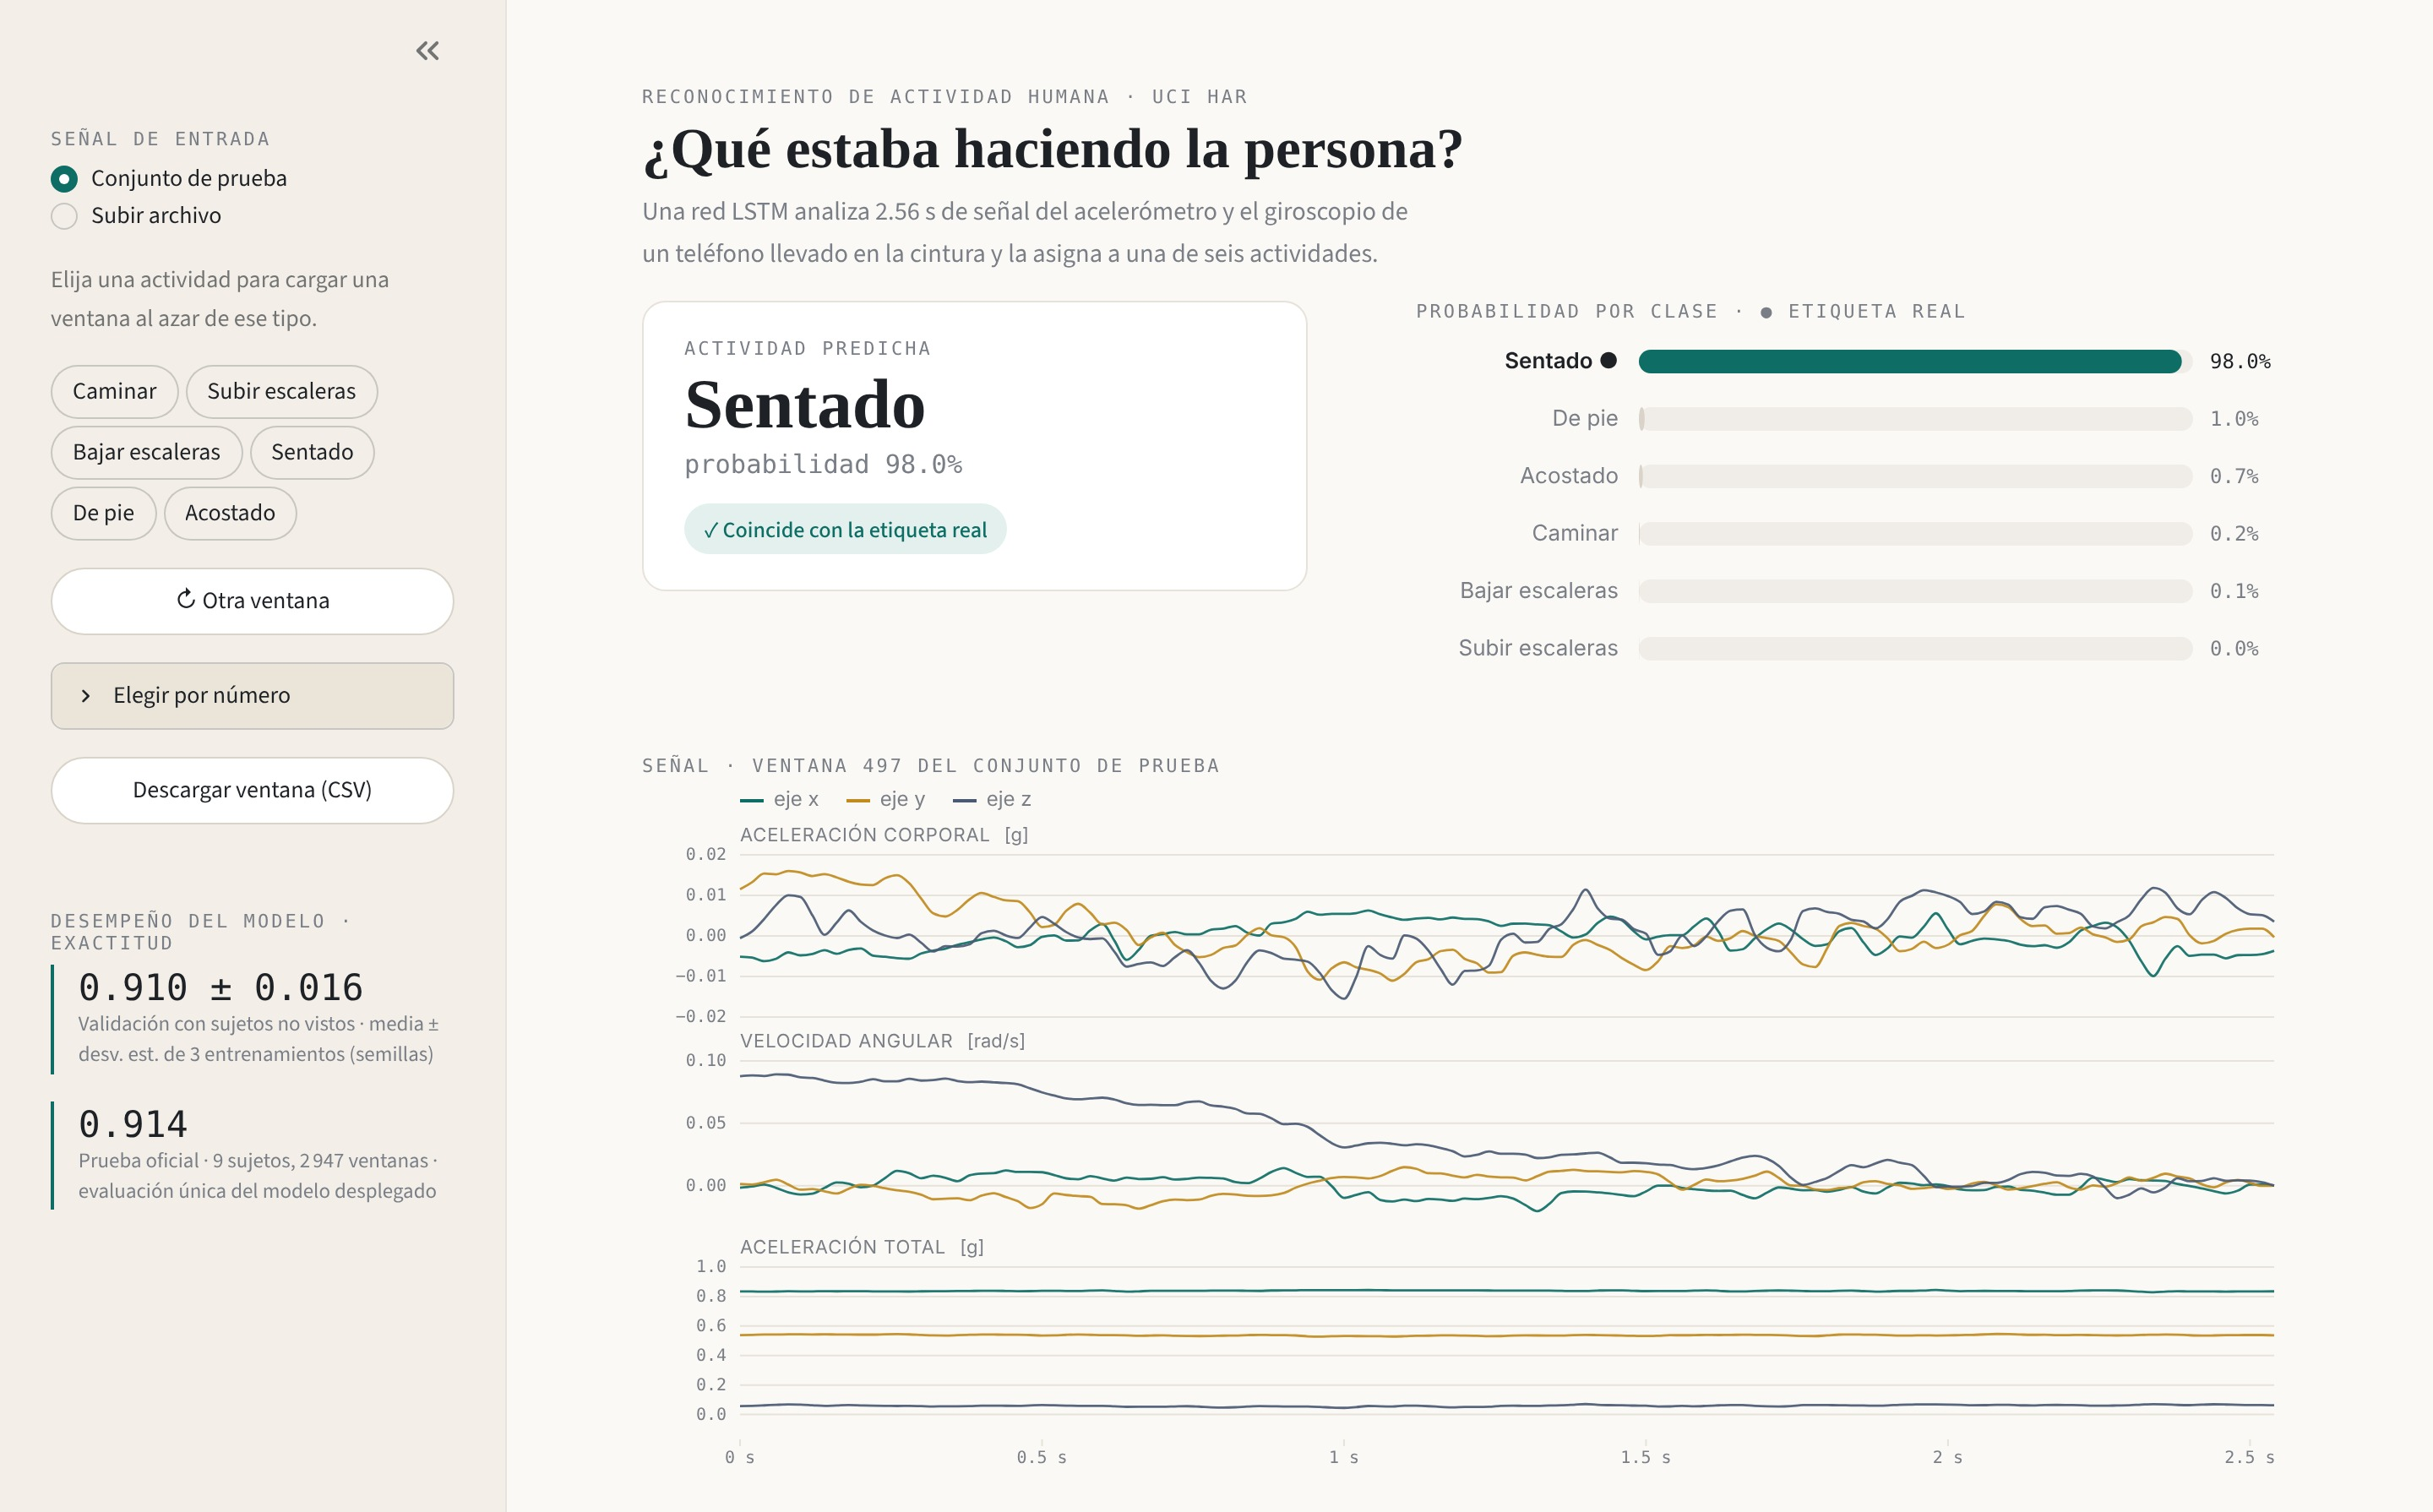
\includegraphics[width=.495\textwidth]{figuras/app_497.jpg}
\caption{Interfaz de clasificación con (a) la ventana 236, \emph{caminar}
(0,976), y (b) la ventana 497, \emph{sentado} (0,980): actividad predicha,
probabilidad por clase (el punto marca la etiqueta real) y señales.}
\label{fig:app}
\end{figure}

% ---------------------------------------------------------------- 6. CONCLUSIONES
\section{Conclusiones}

Una LSTM de 31\,558 parámetros, entrenada sobre señales inerciales crudas con una
partición estrictamente por sujeto, clasificó seis actividades con una exactitud
de 0,910\,$\pm$\,0,016 en validación y de 0,914 en la prueba oficial. La variante
Conv1D+LSTM no mostró una diferencia significativa en ninguno de los dos
protocolos de validación cruzada, por lo que se prefirió el modelo más simple.
El análisis de errores indica que la principal limitación no es la arquitectura
sino la variabilidad entre personas: la confusión entre \emph{de pie} y
\emph{sentado} se concentra en sujetos cuya inclinación del teléfono es atípica,
y una orientación de reposo no vista en entrenamiento produjo errores con alta
confianza.

Los resultados deben leerse con sus limitaciones: solo 17 sujetos de desarrollo
y 4 de validación, un único dispositivo y posición, una validación cruzada de dos
particiones con seis evaluaciones no independientes, un análisis de sensibilidad
con sesgo optimista y una sola semilla evaluada en la prueba. Como trabajo
futuro se proponen el aumento de datos por rotación para obtener invariancia a la
orientación, la calibración de probabilidades, la inclusión de transiciones
posturales etiquetadas y la validación dejando un sujeto fuera.

% ---------------------------------------------------------------- REFERENCIAS
\begin{thebibliography}{7}
\setlength{\itemsep}{0pt}
\small

\bibitem{anguita2013}
Anguita, D., Ghio, A., Oneto, L., Parra, X., Reyes-Ortiz, J.L.: A public domain
dataset for human activity recognition using smartphones. In: Proceedings of the
21st European Symposium on Artificial Neural Networks, Computational Intelligence
and Machine Learning (ESANN 2013), pp. 437--442. Bruges, Belgium (2013)

\bibitem{reyesortiz2012}
Reyes-Ortiz, J., Anguita, D., Ghio, A., Oneto, L., Parra, X.: Human Activity
Recognition Using Smartphones [Dataset]. UCI Machine Learning Repository (2012).
\doi{10.24432/C54S4K}

\bibitem{hochreiter1997}
Hochreiter, S., Schmidhuber, J.: Long short-term memory. Neural Computation
\textbf{9}(8), 1735--1780 (1997). \doi{10.1162/neco.1997.9.8.1735}

\bibitem{ordonez2016}
Ordóñez, F.J., Roggen, D.: Deep convolutional and LSTM recurrent neural networks
for multimodal wearable activity recognition. Sensors \textbf{16}(1), 115 (2016).
\doi{10.3390/s16010115}

\bibitem{hammerla2016}
Hammerla, N.Y., Halloran, S., Plötz, T.: Deep, convolutional, and recurrent
models for human activity recognition using wearables. In: Proceedings of the
25th International Joint Conference on Artificial Intelligence (IJCAI 2016),
pp. 1533--1540 (2016)

\bibitem{bock2022}
Bock, M., Hoelzemann, A., Moeller, M., Van Laerhoven, K.: Investigating
(re)current state-of-the-art in human activity recognition datasets. Frontiers
in Computer Science \textbf{4}, 924954 (2022). \doi{10.3389/fcomp.2022.924954}

\bibitem{nadeau2003}
Nadeau, C., Bengio, Y.: Inference for the generalization error. Machine Learning
\textbf{52}, 239--281 (2003). \doi{10.1023/A:1024068626366}

\end{thebibliography}
\end{document}
